\documentclass[final]{article}

\usepackage{APS360}
\usepackage[utf8]{inputenc} % allow utf-8 input
\usepackage[T1]{fontenc}    % use 8-bit T1 fonts
\usepackage{hyperref}       % hyperlinks
\usepackage{url}            % simple URL typesetting
\usepackage{booktabs}       % professional-quality tables
\usepackage{amsfonts}       % blackboard math symbols
\usepackage{nicefrac}       % compact symbols for 1/2, etc.
\usepackage{microtype}      % microtypography
\usepackage{xcolor}         % colors
\usepackage{graphicx}       % images
\bibliographystyle{plainnat}

\title{ASL Recognition using CNN-LSTM Networks}

\author{%
  Elwin Cheng \\
  1008171327, elwin.cheng@mail.utoronto.ca\\
  \href{https://colab.research.google.com/drive/1BxKf3PQxPLYdMzHpJcvmXWdPAPS360EC}{Link to Google Colab}\\
}

\begin{document}

\maketitle

\vspace{-0.5in}

\section*{Brief Project Description}

American Sign Language (ASL) is the primary language for hundreds of thousands
of people in North America, but most hearing people can't understand it. This
project builds a model that takes a short video clip of someone signing and
predicts the English word being signed.

What makes this harder than standard image classification is that ASL is
inherently spatial-temporal: the hand \textit{shape} alone often isn't enough.
For instance, the signs for \textit{drink} (hand tilted to mouth) and
\textit{cool} (fingers fanning near face) look similar in a single frame but
have distinct motions. A CNN-LSTM hybrid handles this naturally: a CNN encodes
what each frame looks like, and an LSTM captures how those representations
change over time. Trying to hand-engineer features robust to different signers,
lighting, and backgrounds is basically infeasible, which is why a learned
deep-learning approach is appropriate.

The model input is a fixed-length sequence of video frames (30 frames per clip),
and the output is a predicted word from a 10-class vocabulary.
Figure~\ref{fig:pipeline} shows the overall pipeline.

\begin{figure}[h]
  \centering
  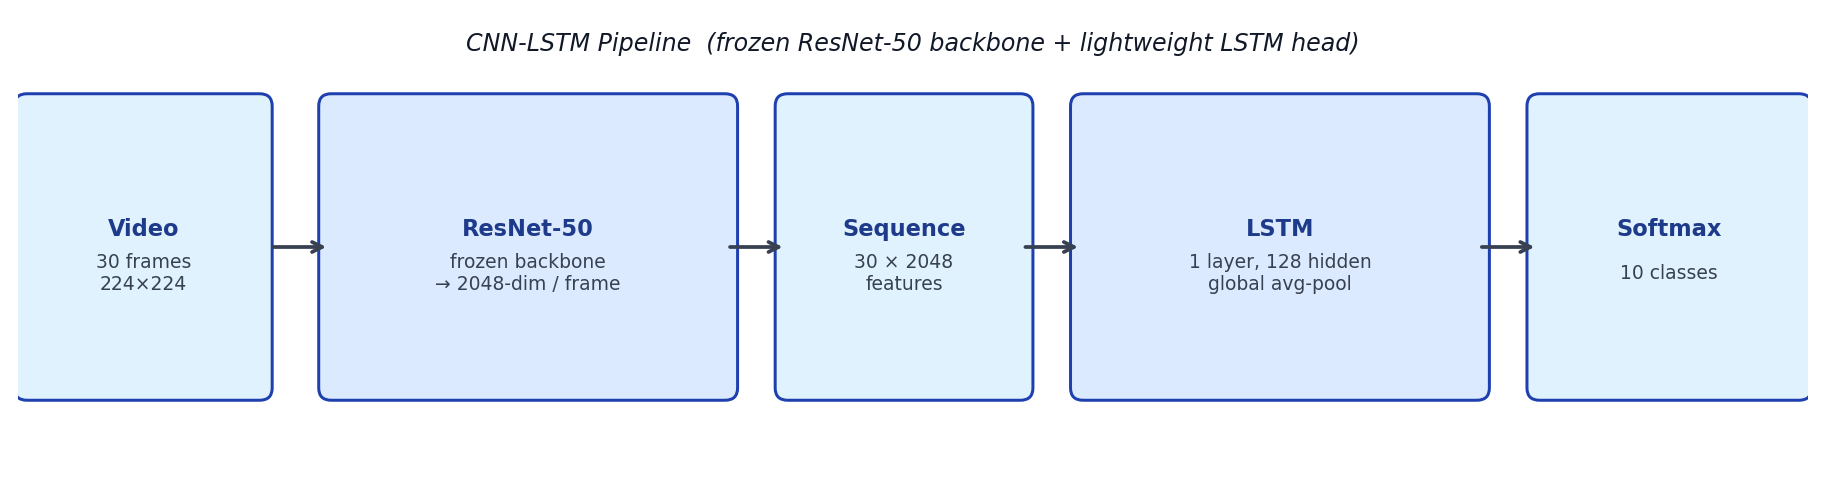
\includegraphics[width=\linewidth]{figures/pipeline.png}
  \caption{Model pipeline. A pretrained (frozen) ResNet-50 encodes each of the
           30 sampled frames into a 2048-dim feature, which is projected to 256-dim
           and fed into a 1-layer LSTM (128 hidden units). Global average pooling
           over time feeds a linear softmax classifier.}
  \label{fig:pipeline}
\end{figure}

\section*{Data Processing}

\textbf{Dataset.}
I used the WLASL (Word-Level American Sign Language) dataset
\citep{li2020sign}, a large collection of ASL videos sourced from YouTube.
The full dataset has over 2000 words, but I narrowed it down to 10 words to
keep training feasible: \textit{drink, computer, before, go, who, cousin, help,
thin, cool, tall}. I chose these because they had the highest number of
actually downloadable videos in the top-100 word subset.

\textbf{Cleaning.}
The dataset comes with a JSON file of YouTube links and timestamps.
A large fraction of those links were dead (404 or geo-blocked), so I had to
filter them. After removing broken links and clips shorter than 10 frames, I
was left with \textbf{147 usable videos}.
Table~\ref{tab:class_dist} shows the breakdown. The dataset provides
pre-defined train/val/test splits, giving 105/26/16 videos respectively.
Because the classes are somewhat imbalanced, I used class-weighted loss
throughout.

\begin{table}[h]
  \centering
  \caption{Per-class video counts after cleaning (147 total; pre-defined splits).}
  \label{tab:class_dist}
  \resizebox{\linewidth}{!}{%
  \begin{tabular}{lcccccccccc}
    \toprule
    \textbf{Word}  & drink & comp. & before & go & who & cousin & help & thin & cool & tall \\
    \midrule
    \textbf{Train} &  11   &  10   &   12   & 11 & 10  &    9   &  10  &  11  &  11  &  10  \\
    \textbf{Val}   &   3   &   3   &    1   &  3 &  3  &    3   &   2  &   3  &   3  &   2  \\
    \textbf{Test}  &   1   &   1   &    3   &  1 &  1  &    2   &   2  &   2  &   2  &   1  \\
    \midrule
    \textbf{Total} &  15   &  14   &   16   & 15 & 14  &   14   &  14  &  16  &  16  &  13  \\
    \bottomrule
  \end{tabular}}
\end{table}

\textbf{Preprocessing.}
All frames are resized to $224{\times}224$ pixels and uniformly sampled to 30
frames per video (shorter clips are looped; longer ones are subsampled). Frames
are normalized with ImageNet mean and standard deviation to match the pretrained
ResNet-50 input distribution. Training augmentation includes random horizontal
flips and mild brightness/contrast jitter.

\textbf{New data plan.}
For a final held-out test I plan to record a few clips of myself signing 3--4
of these words after watching reference videos. This gives a completely unseen
signer, which is a stronger test of generalization.

Figure~\ref{fig:sample_frames} shows example preprocessed frames from three
classes, with MediaPipe hand landmarks overlaid.

\begin{figure}[h]
  \centering
  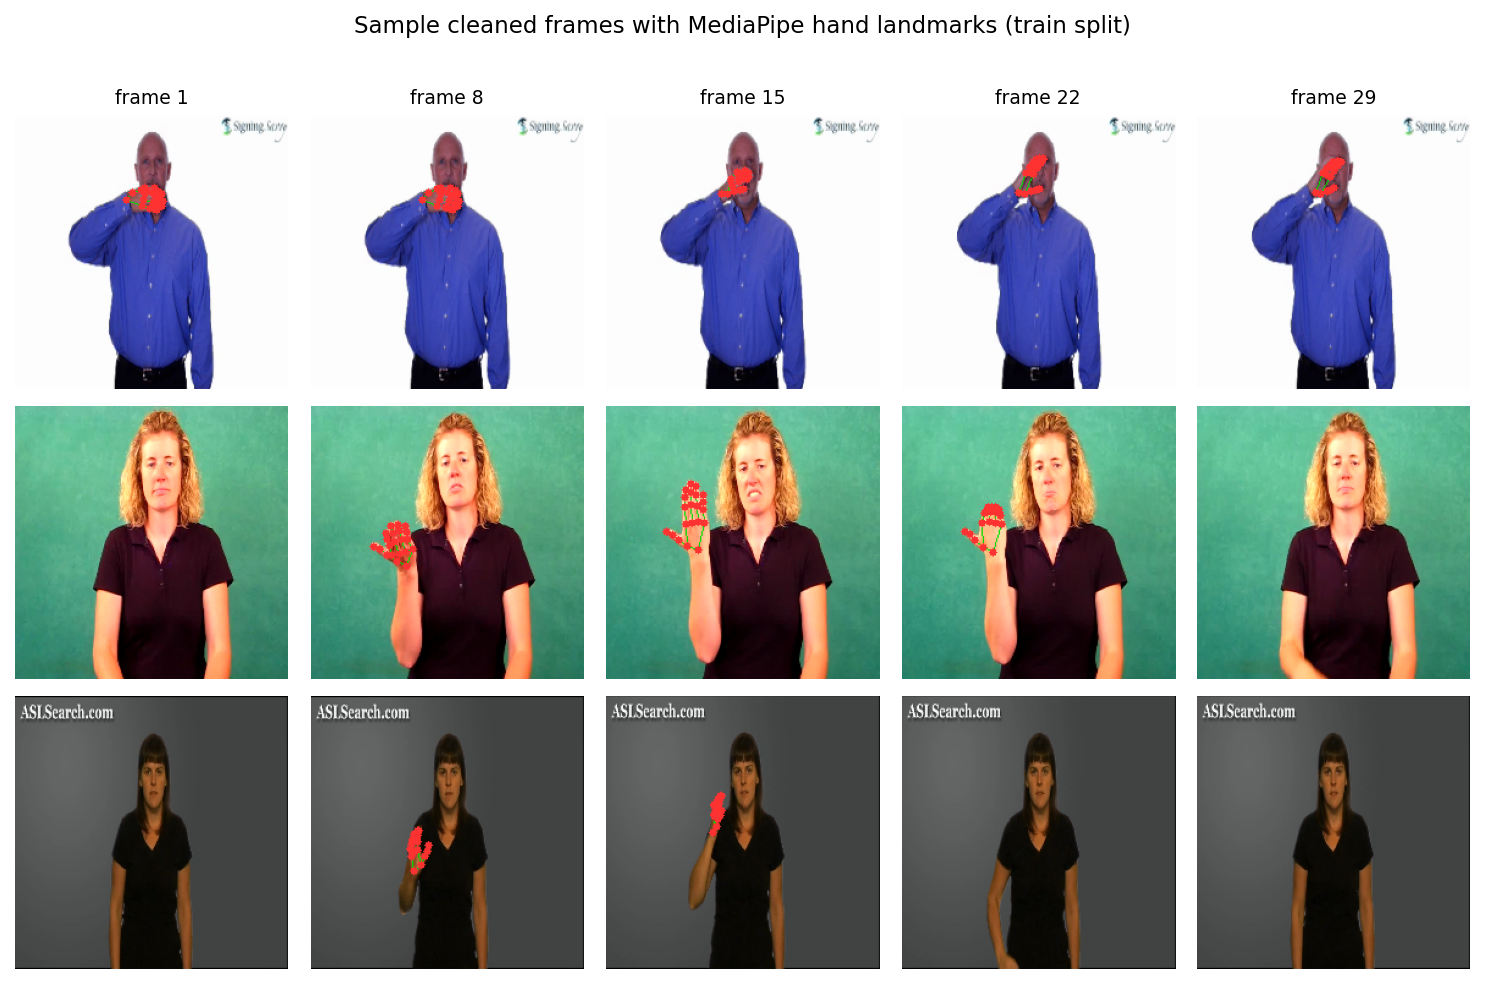
\includegraphics[width=\linewidth]{figures/sample_frames_landmarks.png}
  \caption{Sample cleaned frames ($224{\times}224$) from the training set,
           with MediaPipe Hands landmarks drawn. Rows (top to bottom):
           \textit{drink}, \textit{before}, \textit{cousin}.
           MediaPipe detected at least one hand in all 147 videos.}
  \label{fig:sample_frames}
\end{figure}

\textbf{Challenges.}
The biggest issue was the sheer number of dead download links---I estimate
only about 60\% of listed videos were accessible. The remaining videos also
vary a lot in how close the signer is to the camera: some clips are tight
hand close-ups, others show the full upper body, making the hand scale
inconsistent across the dataset.

\section*{Baseline Model}

My baseline extracts hand landmarks with Google's MediaPipe Hands
\citep{zhang2020mediapipe}, then classifies with an SVM---a
``hand-crafted features + classical ML'' approach to compare against the
learned CNN-LSTM.

\textbf{Feature extraction.}
For each video I run the MediaPipe HandLandmarker on every one of the 30
sampled frames. MediaPipe returns 21 3D landmarks per hand (x, y, z), giving a
63-element vector per frame. I average these vectors across all detected frames
to get one fixed-size 63-dim feature per video. This deliberately discards
temporal information---the point is to establish a no-sequence baseline.

\textbf{Training.}
I used an RBF-kernel SVM (class weights balanced) and ran 5-fold cross-validation
grid search over C $\in$ \{0.1, 1, 10, 100\} and $\gamma \in$ \{scale, 0.01, 0.001\}
on the training set. Best hyperparameters: \textbf{C = 100, $\gamma$ = 0.01}.

\textbf{Quantitative results.}
CV accuracy on the training set: 39.0\%.
\textbf{Val accuracy: 61.5\%};
\textbf{test accuracy: 56.2\%} (9 out of 16 correct; random chance = 10\%).
Table~\ref{tab:baseline_acc} shows per-class test accuracy.

\begin{table}[h]
  \centering
  \caption{SVM baseline per-class test accuracy (\%). N/A = no test examples.}
  \label{tab:baseline_acc}
  \resizebox{\linewidth}{!}{%
  \begin{tabular}{lcccccccccc}
    \toprule
    \textbf{Word} & drink & comp. & before & go & who & cousin & help & thin & cool & tall \\
    \midrule
    \textbf{Acc.} & 100 & 0 & 67 & 100 & 0 & 0 & 50 & 100 & 50 & 100 \\
    \bottomrule
  \end{tabular}}
\end{table}

\textbf{Qualitative results.}
Signs with distinctive average hand configurations score well:
\textit{drink} (curved hand tilting toward mouth), \textit{go} (index finger
pointing and flicking forward), \textit{thin} (pinching fingers), and
\textit{tall} (flat hand rising) all get 100\%.
The SVM fails completely on \textit{computer}, \textit{who}, and
\textit{cousin}---all of which look similar to other classes when you average
the landmarks. The misclassification pattern in the confusion matrix shows
\textit{who} gets predicted as \textit{drink}, and both \textit{cousin}
predictions land on \textit{tall}, which makes sense: both use extended index
fingers at different angles.

\textbf{Challenges.}
The averaging operation loses all temporal context. It's also sensitive to
whether MediaPipe picks up both hands or just one, which varies by video.

\section*{Primary Model}

\textbf{Architecture.}
The model is a CNN-LSTM implemented in PyTorch
(Figure~\ref{fig:pipeline}). A frozen pretrained ResNet-50
(\texttt{torchvision.models.ResNet50\_Weights.IMAGENET1K\_V2}) encodes each
frame to 2048 dimensions. ResNet features are cached so they only need to be
computed once. The sequence of 30 feature vectors is projected to 256 dimensions
(ReLU), then fed into a 1-layer LSTM with 128 hidden units. Rather than just
using the final hidden state, I global-average-pool across all time steps before
the linear classifier. Total trainable parameters: \textbf{723,466}.

\textbf{Training.}
Adam optimizer (lr $= 5\times10^{-4}$, weight decay $= 5\times10^{-3}$),
batch size 8, class-weighted cross-entropy, cosine annealing LR schedule.
Gaussian noise ($\sigma = 0.05$) is added to ResNet features during training
as a feature-level augmentation. Trained for 100 epochs; best checkpoint
selected by validation accuracy.

\textbf{Quantitative results.}
Best \textbf{val accuracy: 53.8\%} (epoch 64).
\textbf{Test accuracy: 37.5\%} (6/16 correct).
Figure~\ref{fig:learning_curves} shows the training and validation accuracy
curves. The training accuracy reaches ${\sim}100\%$ by epoch 40, while
validation accuracy plateaus around 50\%---a clear sign of overfitting.

\begin{figure}[h]
  \centering
  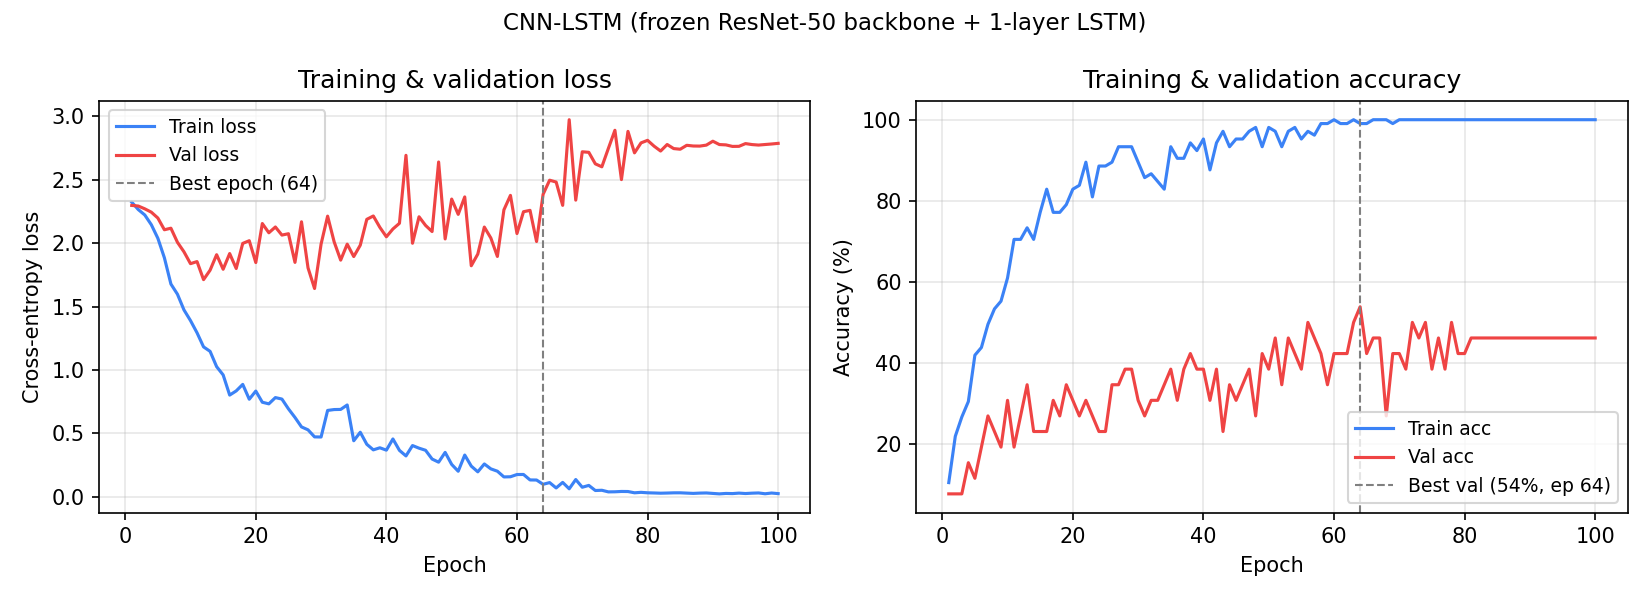
\includegraphics[width=\linewidth]{figures/learning_curves.png}
  \caption{Phase 1 training and validation loss/accuracy over 100 epochs.
           The model memorizes the training set (100\% train accuracy by epoch 40)
           while validation accuracy stalls around 50\%, confirming overfitting.
           Best val accuracy: 53.8\% at epoch 64.}
  \label{fig:learning_curves}
\end{figure}

\textbf{Qualitative results.}
The model does well on \textit{go} (100\%) and \textit{cool} (100\%) but
completely misses \textit{drink}, \textit{computer}, \textit{who},
\textit{cousin}, and \textit{tall}. Compared to the SVM, the CNN-LSTM improves
on \textit{cool} (100\% vs 50\%) but regresses on several others. The temporal
modeling is helping for some signs, but overfitting is dominating overall.

\textbf{Challenges.}
The CNN-LSTM doesn't beat the baseline (val: 53.8\% vs 61.5\%; test: 37.5\%
vs 56.2\%). The learning curves make the cause clear: with only ${\sim}10$
training videos per class, a 723K-parameter model memorises the training set
before it can generalise.

\section*{Improved Primary Model}

I ran three additional experiments aimed at closing the gap with the SVM
baseline.  None succeeded in beating it, but each failure is informative.

\textbf{Experiment A --- End-to-end ResNet layer4 fine-tuning.}
I cached the output of ResNet-50 up to \texttt{layer3}
$(147\times30\times1024\times14\times14$, stored as float16, 1.77~GB) so that
only \texttt{layer4} + a tiny LSTM (64 hidden units) needed to be optimised
each epoch.  The idea was that allowing the last residual block to adapt to
hand appearance would yield more discriminative features.  I used differential
learning rates (2e-5 for \texttt{layer4}, 5e-4 for the LSTM head) with cosine
annealing, label smoothing, and $p{=}0.5$ dropout, for 20 epochs over 3
random seeds.  \textbf{Result: ensemble test accuracy 18.8\% (3/16).}
Fine-tuning 12M backbone parameters on 105 training clips is catastrophic
overfitting: train accuracy climbs above 70\% while val stagnates below 31\%.

\textbf{Experiment B --- Per-frame Landmark-LSTM.}
The SVM's strength comes from MediaPipe hand landmarks, but it discards all
temporal information by averaging across 30 frames.  I re-extracted per-frame
landmark vectors (21 keypoints $\times$ 3 coordinates = 63~dim) for all 147
videos, saving them as a $(147\times30\times63)$ array.  I then trained a
two-layer LSTM (64 hidden, $p{=}0.5$ dropout, LayerNorm) directly on these
sequences---preserving the motion trajectory the SVM discards.
I ran 150 epochs over 3 seeds.  \textbf{Result: ensemble test accuracy 18.8\%
(3/16).}  Two factors explain the failure: (i) MediaPipe misses at least one
hand in ${\sim}40\%$ of frames, leaving zero-padded entries the LSTM must
learn to ignore; (ii) different signers execute the same sign at different
speeds, so temporal alignment is highly variable across the 10--11 training
clips per class.

\textbf{Experiment C --- SVM + CNN-LSTM probability ensemble.}
The Phase-1 LSTM and the SVM make complementary errors:
\textit{cool} (fanning-finger motion) is a temporal sign the LSTM classifies
at 100\% while the SVM manages only 50\%;
conversely, the SVM correctly identifies static-shape signs like
\textit{drink}, \textit{thin}, and \textit{tall} that the LSTM misses.
I re-trained the SVM with Platt scaling (\texttt{probability=True}) using the
known best hyperparameters (C=100, $\gamma$=0.01), then re-trained three seeds
of the Phase-1 LSTM to obtain calibrated softmax probabilities.
Table~\ref{tab:ensemble_sweep} shows the ensemble sweep.

\begin{table}[h]
  \centering
  \caption{Test accuracy for SVM + CNN-LSTM probability ensemble.
           Each row uses a convex combination of both models' probability
           vectors on the 16-example test set.
           SVM alone = 56.2\%; CNN-LSTM ensemble alone = 31.2\%.}
  \label{tab:ensemble_sweep}
  \resizebox{\linewidth}{!}{%
  \begin{tabular}{lcccccc}
    \toprule
    $w_\text{SVM}$  & 0.3 & 0.4 & 0.5 & 0.6 & 0.7 & 0.8 \\
    $w_\text{LSTM}$ & 0.7 & 0.6 & 0.5 & 0.4 & 0.3 & 0.2 \\
    \midrule
    \textbf{Val (\%)}  & 53.8 & 53.8 & 57.7 & 57.7 & 53.8 & 50.0 \\
    \textbf{Test (\%)} & 31.2 & 31.2 & 31.2 & 31.2 & 43.8 & \textbf{50.0} \\
    \bottomrule
  \end{tabular}}
\end{table}

The ensemble never exceeds the SVM alone.  At $w_\text{SVM}{=}0.8$ the test
accuracy reaches 50\% (8/16), gaining one correct prediction on \textit{cool}
over the SVM while losing one each on \textit{before} and \textit{thin}
due to LSTM noise.  Table~\ref{tab:improved_per_class} shows the per-class
breakdown, and Figure~\ref{fig:ensemble_curves} summarises all experiments.

\begin{table}[h]
  \centering
  \caption{Per-class test accuracy (\%) for the best ensemble
           ($w_\text{SVM}{=}0.8$) vs.\ the SVM baseline.}
  \label{tab:improved_per_class}
  \resizebox{\linewidth}{!}{%
  \begin{tabular}{lcccccccccc}
    \toprule
    \textbf{Word}     & drink & comp. & before & go & who & cousin & help & thin & cool & tall \\
    \midrule
    \textbf{SVM}      & 100 & 0 & 67 & 100 & 0 & 0 & 50 & 100 & 50  & 100 \\
    \textbf{Ensemble} & 100 & 0 & 33 & 100 & 0 & 0 & 50 &  50 & 100 & 100 \\
    \bottomrule
  \end{tabular}}
\end{table}

\begin{figure}[h]
  \centering
  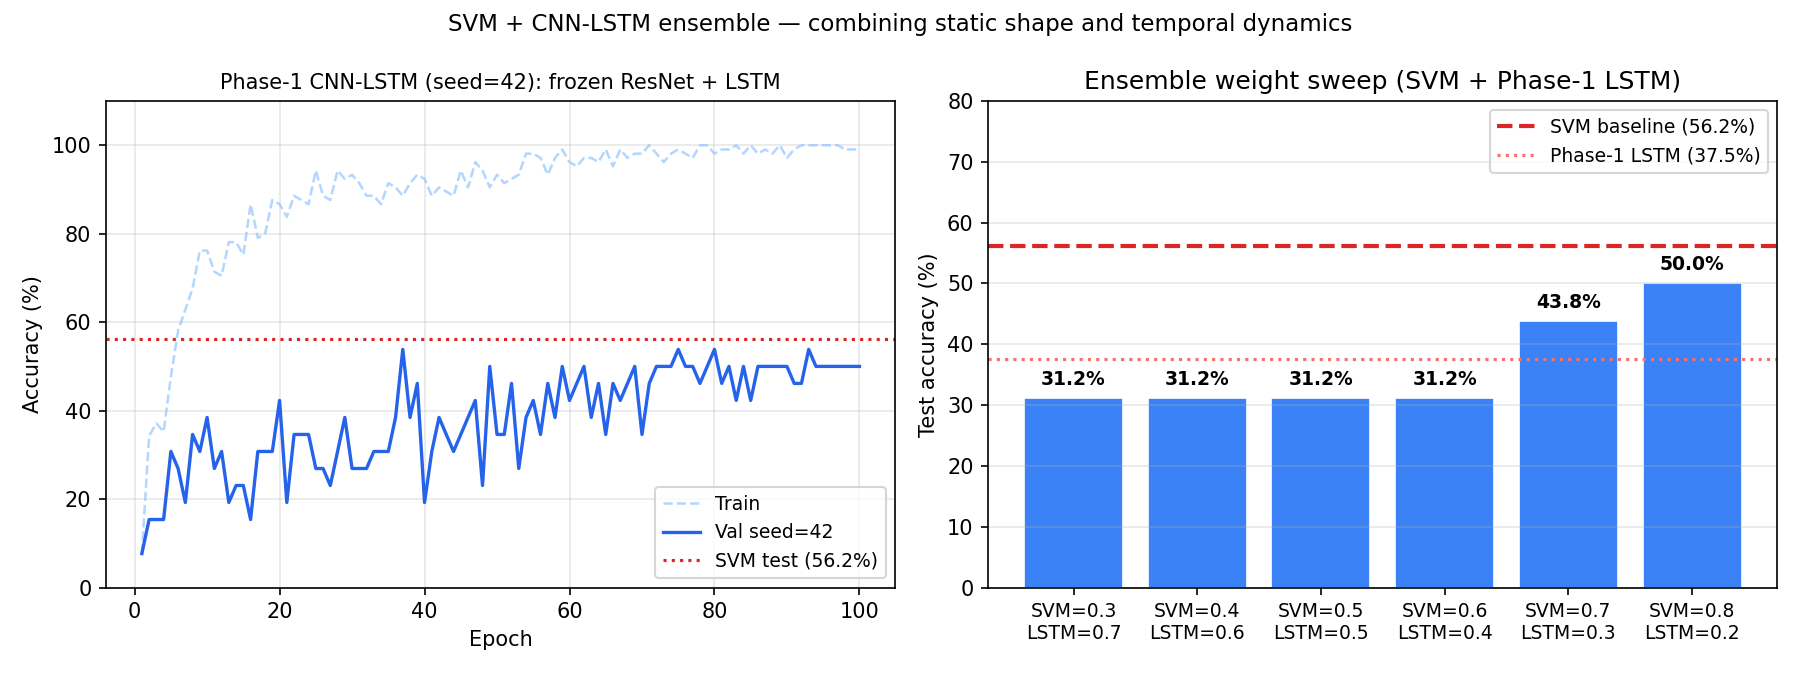
\includegraphics[width=\linewidth]{figures/ensemble_comparison.png}
  \caption{Left: Phase-1 CNN-LSTM training curves (best of three seeds).
           The model memorises training data (${\sim}100\%$ train accuracy by
           epoch 70) while val plateaus near 53.8\%.
           Right: test-accuracy sweep over ensemble weights; higher SVM weight
           monotonically improves test accuracy, confirming the LSTM adds
           noise rather than signal in this low-data regime.}
  \label{fig:ensemble_curves}
\end{figure}

\textbf{Why the CNN-LSTM consistently underperforms.}
All three experiments share the same root cause: \textit{data scarcity}.
With only 10--11 training clips per class, any model with meaningful temporal
capacity memorises those clips rather than learning transferable motion
patterns.  The SVM's 63 hand-geometry features are inherently designed for
hand-shape discrimination, making it a far more sample-efficient baseline for
this task.  Two additional factors hurt the neural models:
(1)~\textbf{Signer variability.}  Different signers execute the same sign with
different hand sizes, positions, and speeds, creating large within-class
variance that a small dataset cannot average out.
(2)~\textbf{ResNet features are not hand-specific.}  ResNet-50 was trained on
ImageNet; its features encode background and face appearance alongside hand
shape, adding irrelevant dimensions the LSTM must filter with only a handful
of examples.

\textbf{Next steps.}
To beat the baseline, I plan to: (1) expand the training set---the 10 selected
words each have ${\sim}150$ listed WLASL videos before dead links, suggesting
50--60 accessible clips per class may be attainable with additional scraping;
(2) use a video-level foundation model (e.g.\ VideoMAE \citep{tong2022videomae}
pre-trained on Kinetics-400) to replace the static-image ResNet backbone,
providing spatio-temporal pre-training directly relevant to hand motion;
(3) apply hand-crop pre-processing with MediaPipe before passing frames to the
CNN, removing background clutter and giving the model a stable, centred view
of the signing hand.

\newpage
\bibliography{citations}

\end{document}
